

\subsection{Visualization of Kinetic Data Structures}
\label{sec:kds_delaunay_2_example}

The framework includes Qt widgets for displaying kinetic data
structures in two and three dimensions. The following example shows
using the two dimensional widget with a Delaunay triangulation:

\begin{ccExampleCode}
#include <CGAL/Kinetic/Exact_simulation_traits_2.h>
#include <CGAL/Kinetic/Delaunay_triangulation_2.h>
#include <CGAL/Kinetic/Enclosing_box_2.h>
#include <CGAL/Kinetic/IO/Qt_moving_points_2.h>
#include <CGAL/Kinetic/IO/Qt_triangulation_2.h>
#include <CGAL/Kinetic/IO/Qt_widget_2.h>

int main(int argc, char *argv[]) {
    using namespace CGAL::Kinetic;
    typedef Exact_simulation_traits_2 Traits;
    typedef Delaunay_triangulation_2<Traits> Del_2;
    typedef Enclosing_box_2<Traits> Box_2;
    typedef Qt_widget_2<Traits::Simulator> Qt_widget;
    typedef Qt_moving_points_2<Traits, Qt_gui> Qt_mps;
    typedef Qt_triangulation_2<Del_2, Qt_widget, Qt_mps> Qt_dt2;
    
    // create a simulation traits and add two KDSs:
    // a kinetic Delaunay triangulation and an enclosing box;
    // the moving points bounce against the walls of the enclosing box
    Traits tr;
    Box_2::Handle box = new Box_2(tr);
    Del_2::Handle kdel = new Del_2(tr);

    // register the simulator, set of moving points and
    // Delaunay triangulation with the kinetic Qt widget
    Qt_widget::Handle qt_w = new Qt_widget(argc, argv, tr.simulator_handle());
    Qt_mps::Handle qt_mps = new Qt_mps(qt_w, tr);
    Qt_dt2::Handle qt_dt2 = new Qt_dt2(kdel, qt_w, qt_mps);

    // read the trajectories of the moving points
    //  the simulation traits automatically inserts them in the two KDSs
    // and schedules the appropriate kinetic events; as in the kinetic
    // sorting example this is done with appropriate notifications
    std::ifstream in("data/points_2");    
    in  >> *tr.active_points_2_table_handle();

    // run the interactive kinetic simulation
    return qt_w->begin_event_loop();
};
\end{ccExampleCode}

The example shows how to use a number of additional features of the
framework. First, it shows that two kinetic data structures
(\ccc{Kinetic::Delaunay_triangulation_2<Traits, Triangulation>} and
\ccc{Kinetic::Enclosing_box_2<Traits>}) can coexist on the same set of
points without any extra effort. Both interact with the moving points
through the active objects table, and never need to directly interact
with one another. Second, objects (like
\texttt{qt\_w}, \texttt{qt\_mps} and \texttt{qt\_dt2}) are all stored
by using reference counted handles (\texttt{Object::Handle}). This
allows them to share references to one another without the user having
to worry about memory management and order of deletion.  For example,
the \ccc{Kinetic::Qt_triangulation_2<KineticDelaunay_2, QtWidget_2,
Qt_moving_points_2>} object needs a handle to the kinetic
triangulation, in order to get the structure to display, and a handle
to the \ccc{Active_points_1_table} to get the coordinates of the
points.


Finally, the example shows how to use the graphical interface elements
provided, see Figure~\ref{fig:kds_qtwidget_capture}. Our package includes
\texttt{Qt} widgets for displaying kinetic geometry in two and three
dimensions. In addition to being able to play and pause the
simulation, the user can step through events one at a time and reverse
the simulation to retrace what had happened. The three-dimensional
visualization support is based on the Coin library http://www.coin3d.org.

\begin{figure*}[htb]
\begin{ccTexOnly}
\begin{center}
1.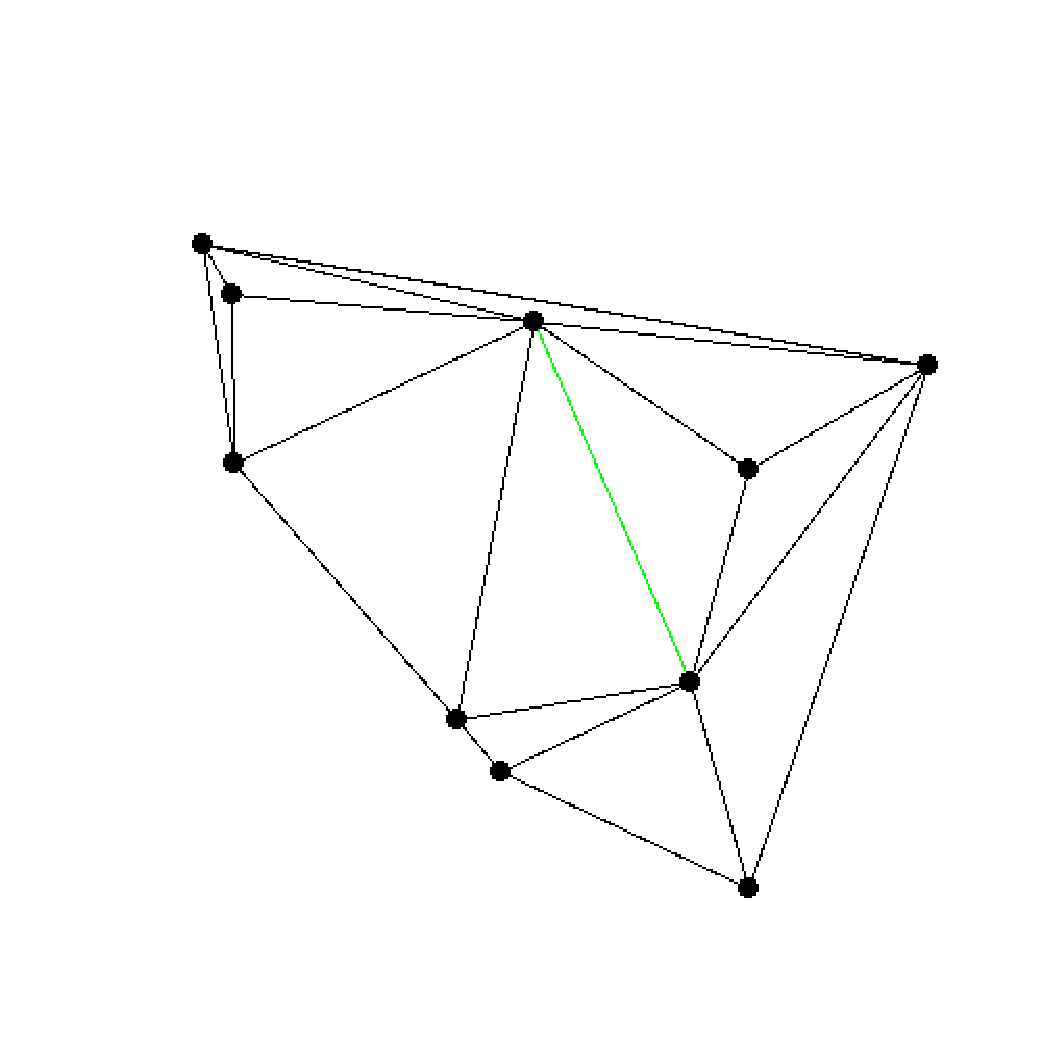
\includegraphics[ scale=.2]{Kinetic_data_structures/delaunay_0} 
2.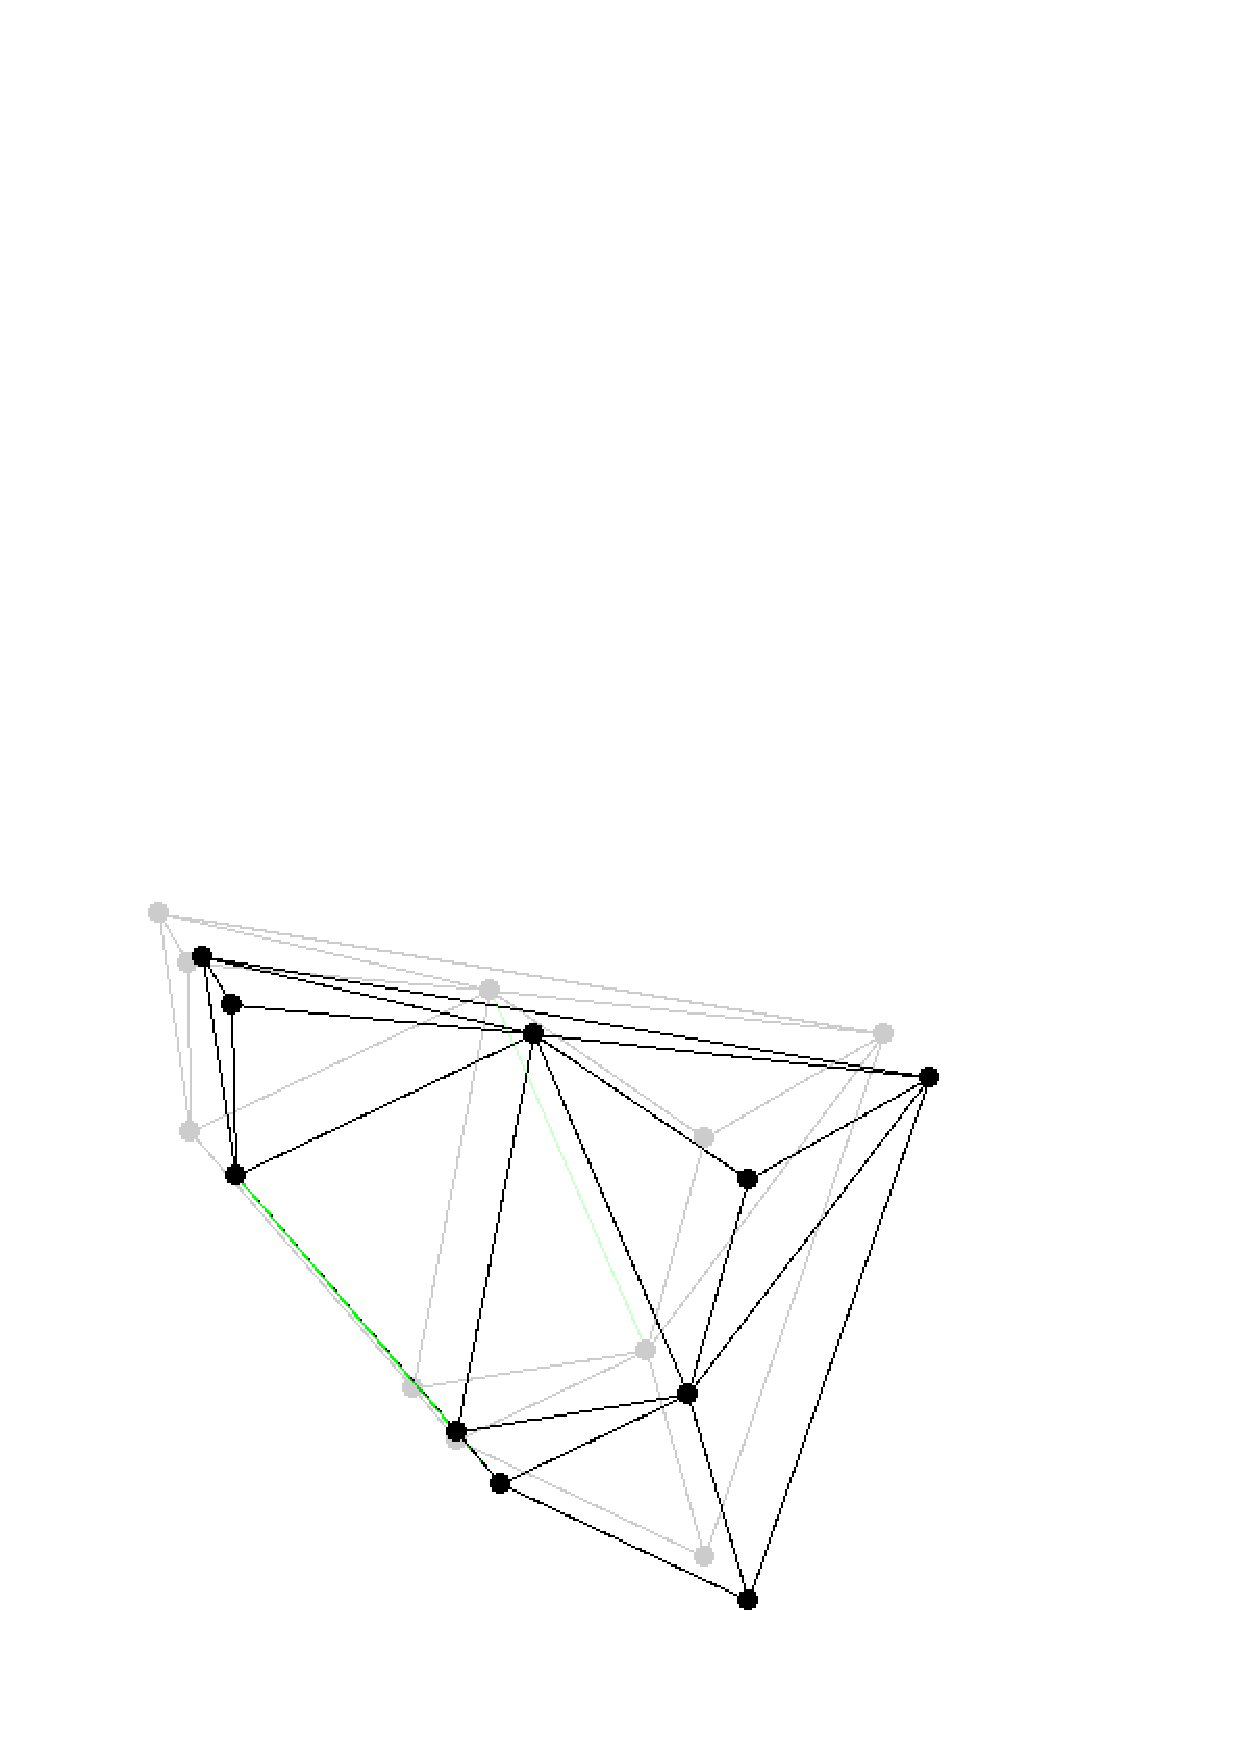
\includegraphics[ scale=.2]{Kinetic_data_structures/delaunay_1}
3.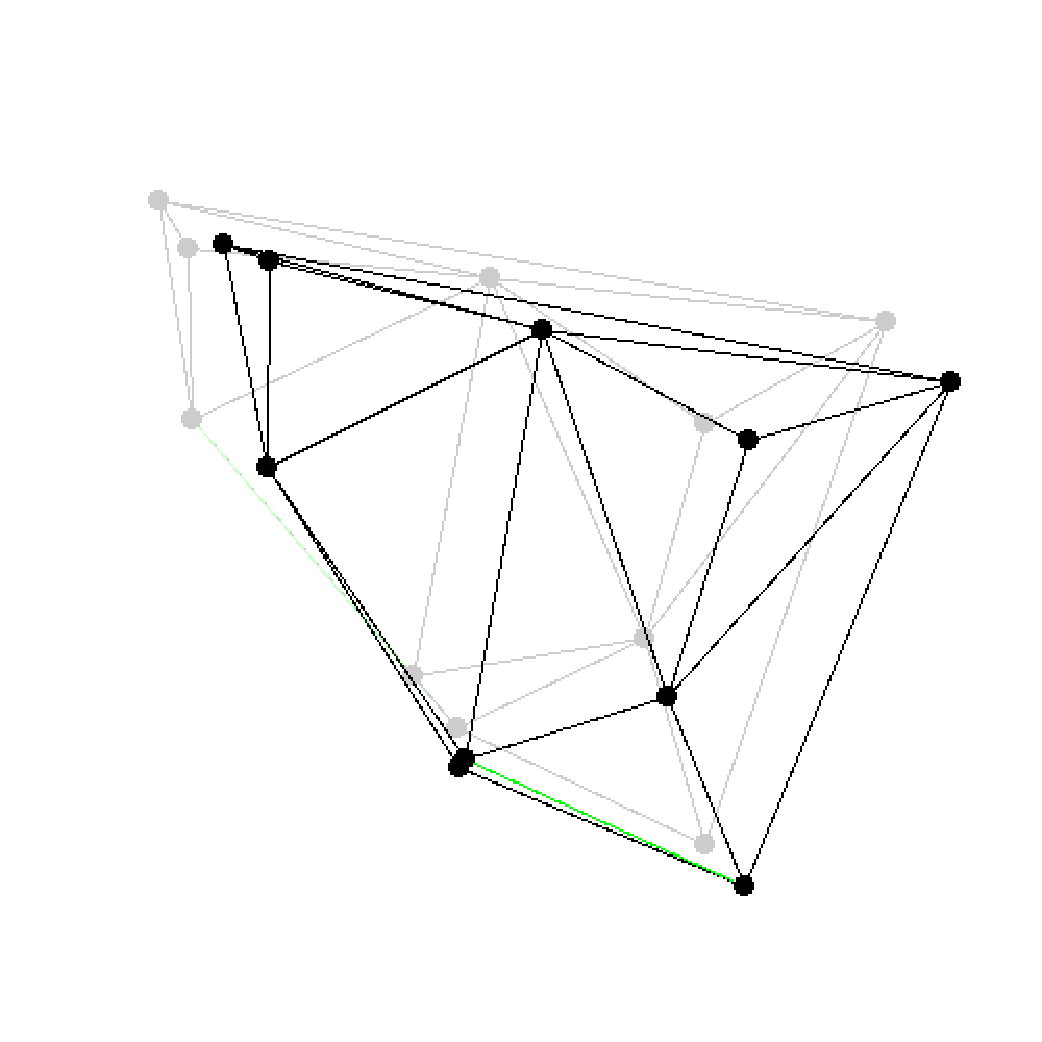
\includegraphics[ scale=.2]{Kinetic_data_structures/delaunay_2}\\
4.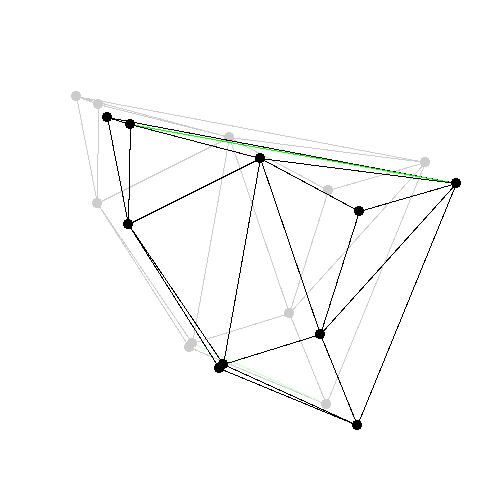
\includegraphics[ scale=.2]{Kinetic_data_structures/delaunay_3}
5.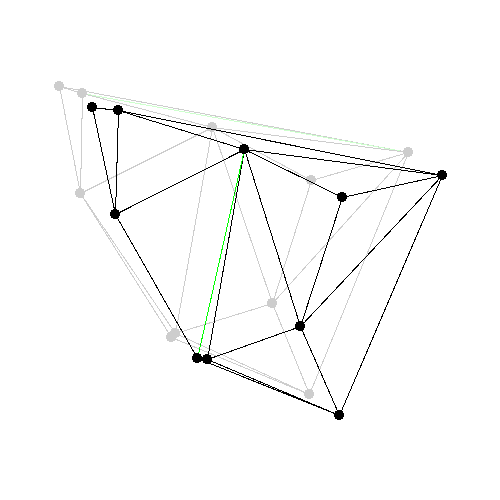
\includegraphics[ scale=.2]{Kinetic_data_structures/delaunay_4}
6.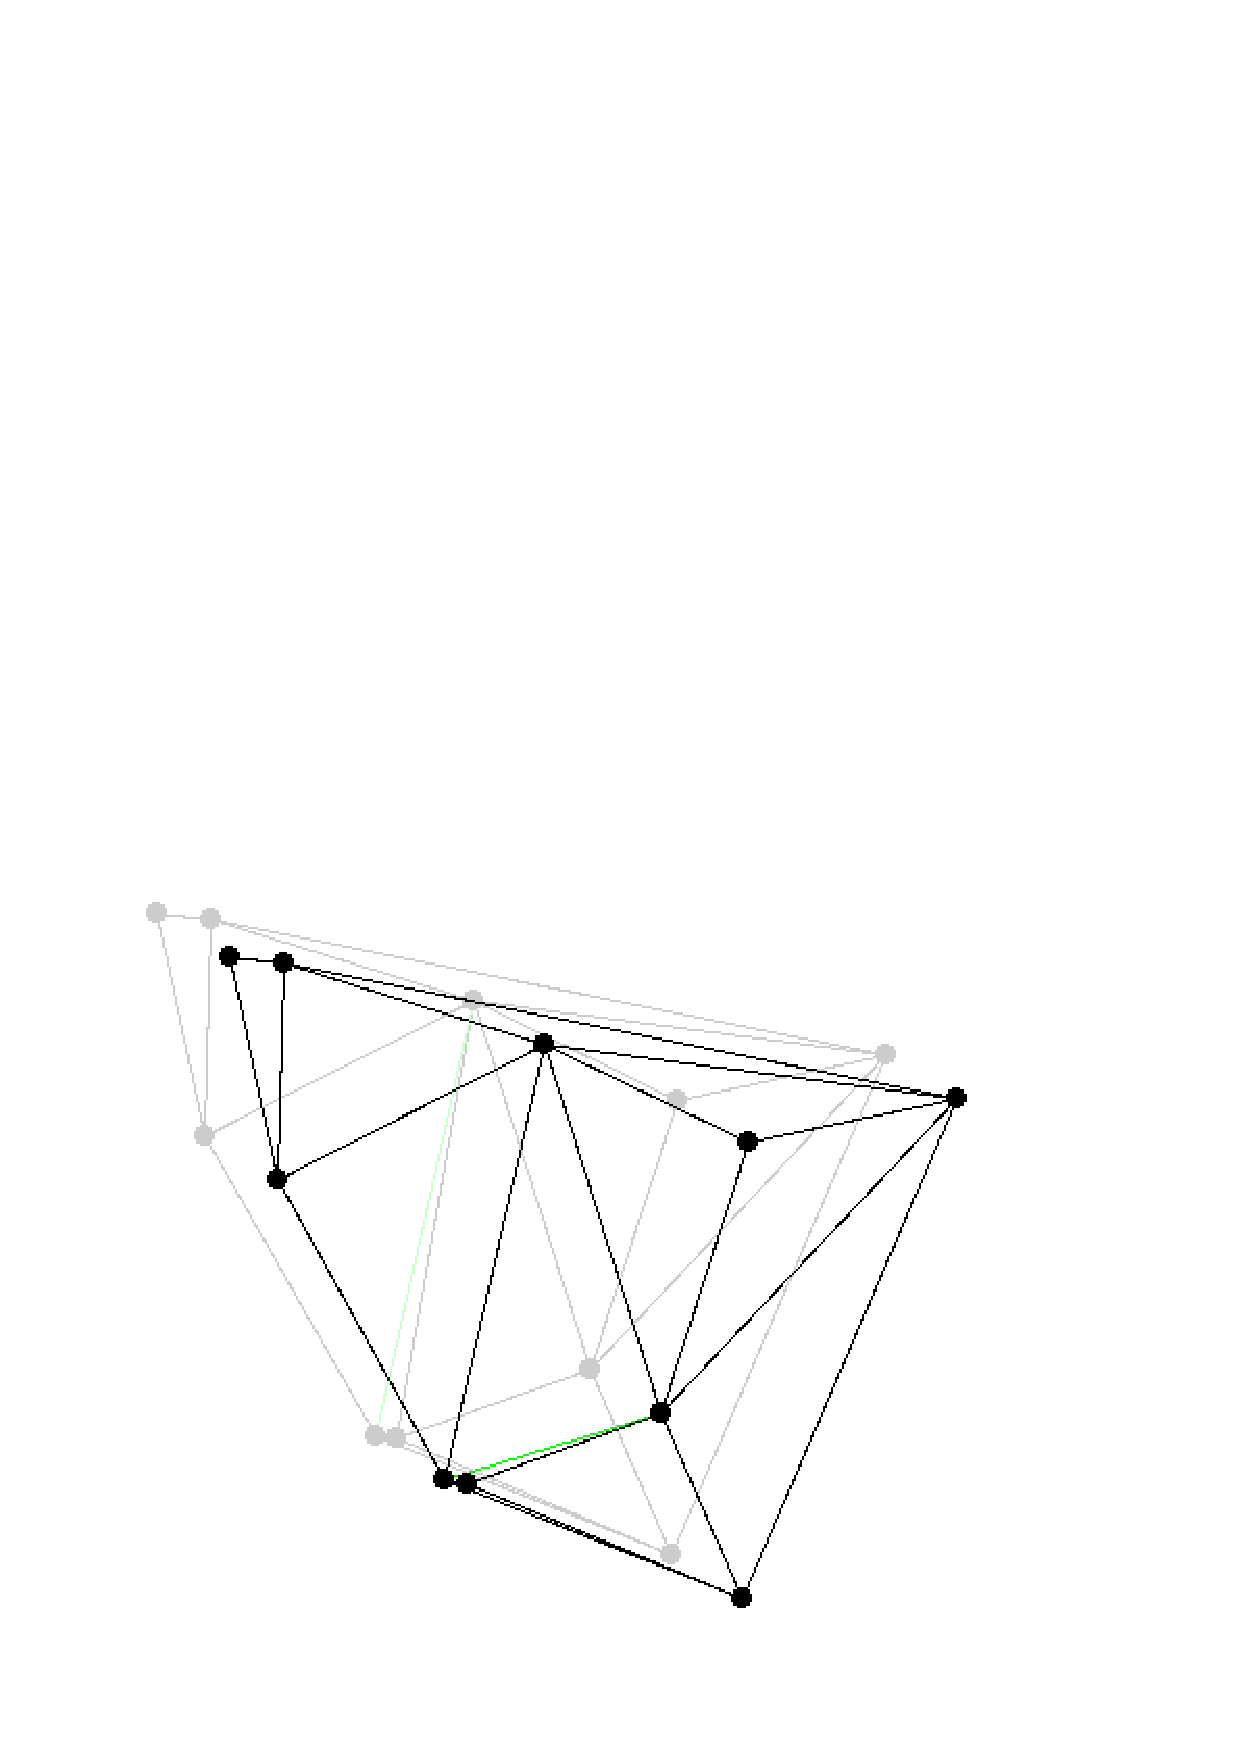
\includegraphics[ scale=.2]{Kinetic_data_structures/delaunay_5}\\
7.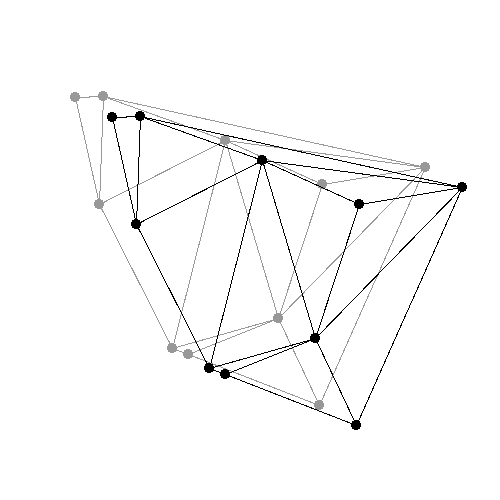
\includegraphics[ scale=.2]{Kinetic_data_structures/delaunay_6}
8.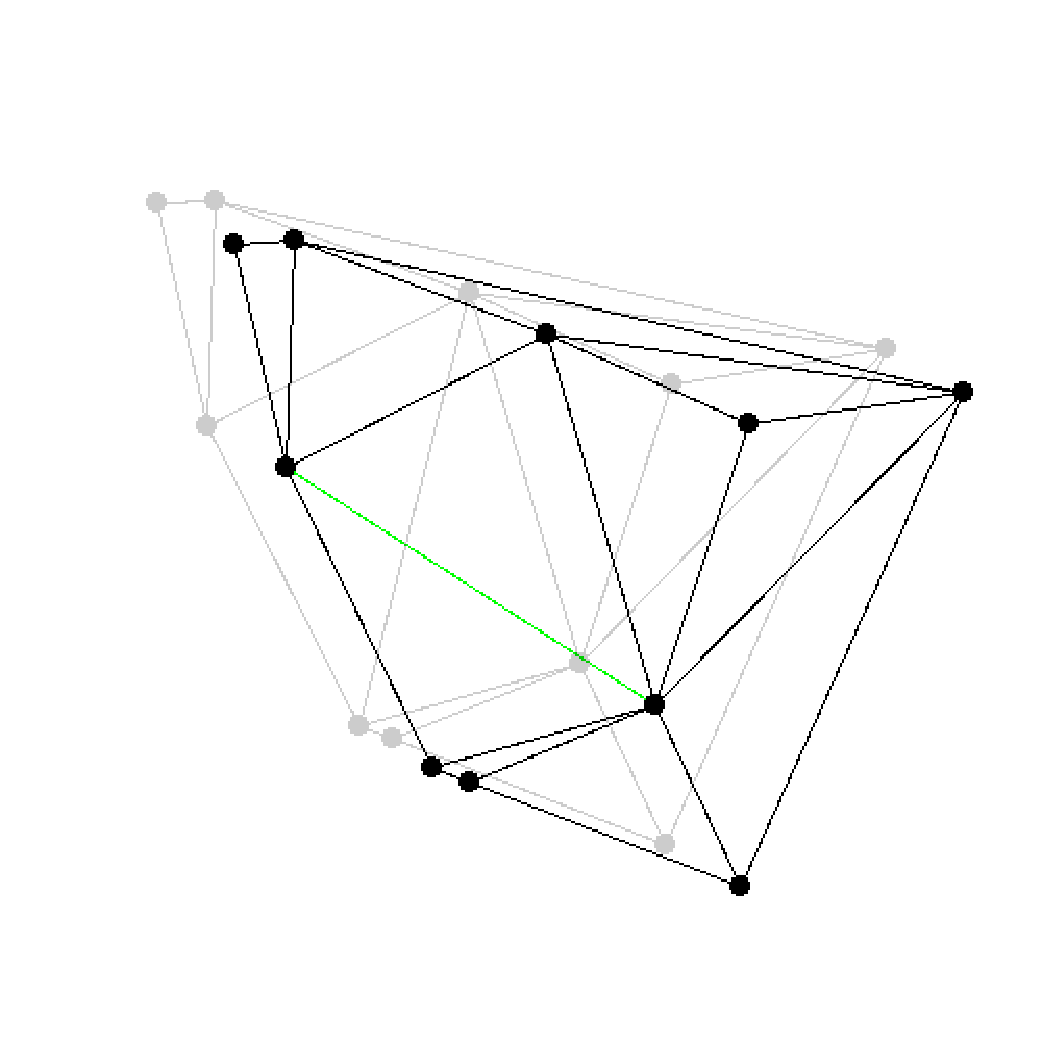
\includegraphics[ scale=.2]{Kinetic_data_structures/delaunay_7}
9.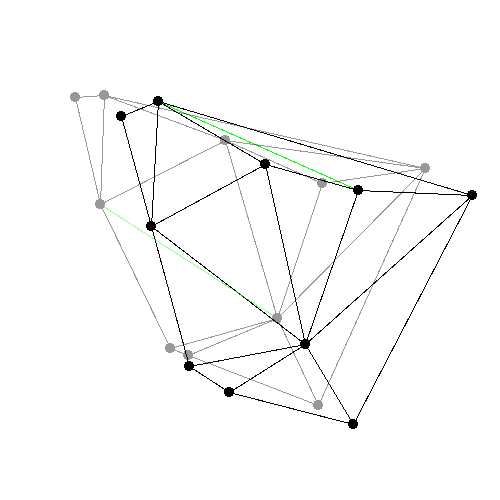
\includegraphics[ scale=.2]{Kinetic_data_structures/delaunay_8}
\end{center}
\end{ccTexOnly}
%width=300 height=300
\begin{ccHtmlOnly}

<img border=1 src="./delaunay_0.gif" align=center alt="Frame 0" >
<img border=1 src="./delaunay_1.gif" align=center alt="Frame 1" >
<img border=1 src="./delaunay_2.gif" align=center alt="Frame 2" >
<img border=1 src="./delaunay_3.gif" align=center alt="Frame 3" >
<img border=1 src="./delaunay_4.gif" align=center alt="Frame 4" >
<img border=1 src="./delaunay_5.gif" align=center alt="Frame 5" >
<img border=1 src="./delaunay_6.gif" align=center alt="Frame 6" >
<img border=1 src="./delaunay_7.gif" align=center alt="Frame 7" >
<img border=1 src="./delaunay_8.gif" align=center alt="Frame 8" >
<br>
\end{ccHtmlOnly}
\caption{ \label{fig:kds_delaunay_events} 
{\em Some events from a Delaunay triangulation kinetic data
structure:} The state of the two dimensional Delaunay triangulation
immediately following the first events is shown. Green edges are ones
which were just created. The pictures are screen shots from
demo/Kinetic\_data\_structures/Delaunay\_triangulation\_2.C. }
%\end{minipage}
%\end{center}
\end{figure*}


\begin{figure}
\begin{ccTexOnly}
\begin{center}
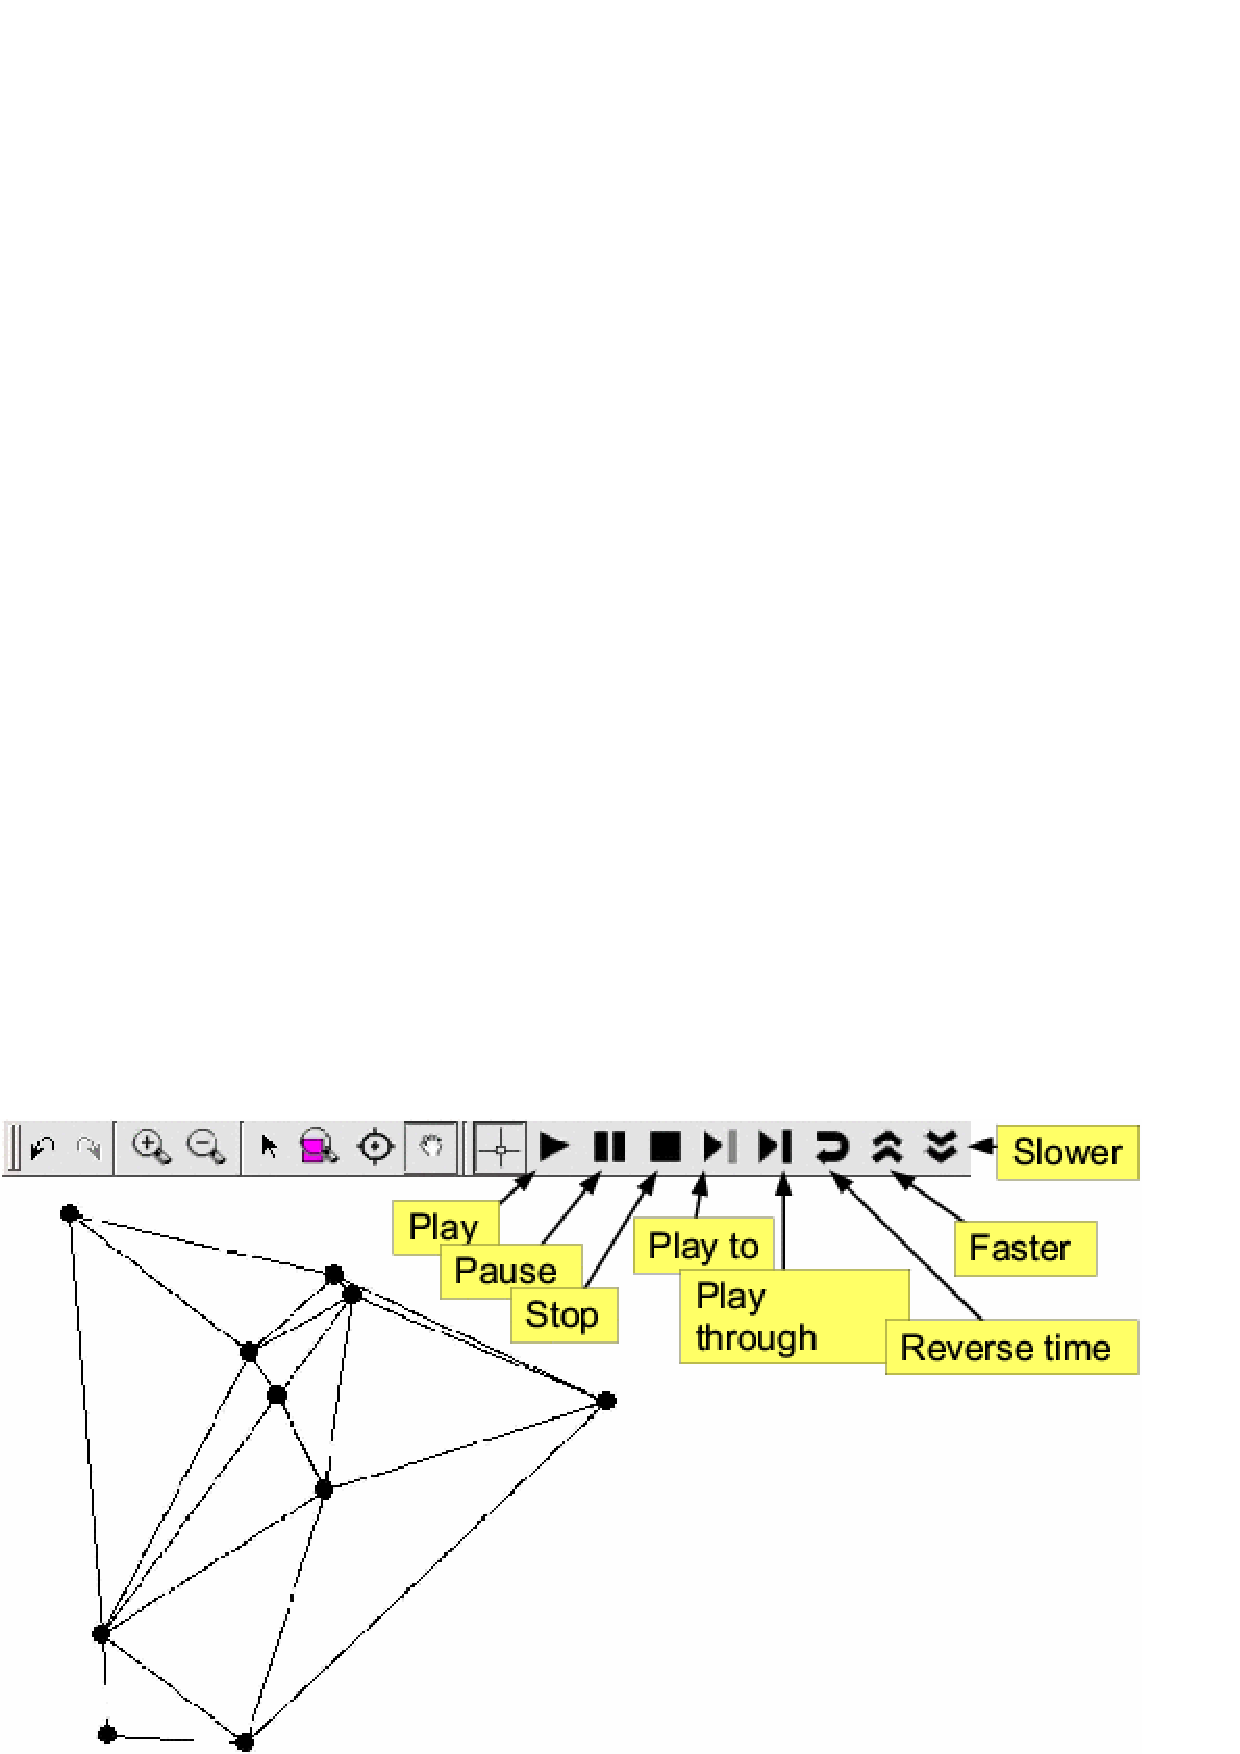
\includegraphics[scale=.5]{Kinetic_data_structures/qt_widget_marked_pct}
\end{center}
\end{ccTexOnly}
\begin{ccHtmlOnly}
<img src="./qt_widget_marked_pct.gif" align=center alt="Qt widget"> <br>
\end{ccHtmlOnly}
\caption{\label{fig:kds_qtwidget_capture} The figure shows the graphical user interface for
  controlling two-dimensional kinetic data structures. It is built on
  top of the \ccc{Qt_widget} and adds buttons to play, pause, step
  through and run the simulation backwards.}
\end{figure}
